\documentclass[12pt]{article}
\usepackage[margin=1in]{geometry}
\usepackage{amsmath,amssymb}
\usepackage{graphicx}
\usepackage{hyperref}
\usepackage{enumitem}
\usepackage{caption}
\usepackage{setspace}
\onehalfspacing
\graphicspath{{../../static/screenshots/}}

\title{专利一：多源协同量子时序检测与风险评估方法与系统}
\author{申请人：ChainAML 项目}
\date{\today}

\begin{document}
\maketitle

\begin{abstract}
提出一种面向区块链交易的反洗钱检测方法及系统，通过时间共振检测识别协同尖刺与周期性异常，引入哈希链金丝雀水印并以量子态保真度进行可验证追踪，融合喷洒/漏斗/混币/挖矿/量子等五类检测分数进行风险评估与分类，提高检出率与取证可解释性。
\end{abstract}

\section*{技术领域}
本发明属于区块链反洗钱、时间序列分析与量子计算交叉领域。

\section*{背景技术}
在协同交易与批量转移场景，传统单一规则模型易被规避，缺乏可信、可验证的证据链支撑审计与合规要求。

\section*{发明内容（概要）}
本方法构建时间共振检测、金丝雀水印与量子态验证、五类融合评估的闭环检测框架，输出交易级风险与分类概率分布，实现可解释的反洗钱检测。

\section*{附图说明}
图1：总体流程图（四步流程与融合模块）。\\
图2：结果展示示意（步骤IV圆环图——五类分布、交易风险表）。\\
图3：页面截图——Step I（时间尖刺）与 Step II（黏菌网络）占位。\\
图4：页面截图——Step III（量子干涉）与 Step IV（分类环图）占位。\\
图5：分类列表页面截图占位。

\section*{具体实施方式}
\subsection*{实施环境与数据集}
操作系统：macOS；后端：Flask。主要接口：\texttt{/api/detections}、\texttt{/api/detection/<type>}、\texttt{/api/transaction/<tx\_id>}。页面：\texttt{index.html}、\texttt{index2.html}、\texttt{AML.html}、\texttt{detail.html}、\texttt{classification.html}。数据集：\texttt{data/sample\_txs.json}（或 \texttt{sample/sample\_txs.json}），字段 \texttt{tx\_id, ts, from, to, amount}。

\subsection*{时间分桶与 Z 分数检测}
将时间轴离散为桶 $B_k$，计数 $x_k=|\{tx\in B_k\}|$；均值与标准差：
\begin{equation}
\mu=\frac{1}{K}\sum\limits_{k}x_k,\quad \sigma=\sqrt{\frac{1}{K}\sum\limits_{k}(x_k-\mu)^2}
\end{equation}
尖刺检测：
\begin{equation}
z_k=\frac{x_k-\mu}{\sigma},\ \ \text{若}\ \ z_k\ge z_{\mathrm{thr}}\ \text{则判定异常}
\end{equation}

\subsection*{周期性共振（频域）}
对序列进行 FFT：$X(f)=\mathrm{FFT}(x_k)$；若存在显著峰 $|X(f_0)|\ge \theta$，视为周期协同共振。

\subsection*{金丝雀水印与量子验证}
哈希链：
\begin{equation}
h_0=\mathrm{SHA3}(seed),\ \ h_{i+1}=\mathrm{SHA3}(h_i\Vert tx_i)
\end{equation}
量子态（幅度编码）：
\begin{equation}
|\psi\rangle=\sum\limits_{i}w_i|i\rangle,\ \ w_i=\mathrm{normalize}(h_i)
\end{equation}
保真度：
\begin{equation}
F=|\langle \psi_{\text{expected}}|\psi_{\text{observed}}\rangle|^2,\ \ \text{若}\ F\ge F_{\mathrm{thr}}\ \text{则水印有效}
\end{equation}

\subsection*{五类风险融合与量子修正}
融合：$R=\sum\limits_{m} w_m\cdot s_m$；量子修正：
\begin{equation}
R'=\alpha R+(1-\alpha)p_q
\end{equation}

\subsection*{数据字段示例}
\begin{verbatim}
{
  "tx_id": "tx_9997_1761288861",
  "ts": 1761288861,
  "from": "0xabc...",
  "to": "0xdef...",
  "amount": 4.2,
  "risk_score": 0.86,
  "detection_type": ["spray", "quantum"]
}
\end{verbatim}

\section*{权利要求书}
\begin{enumerate}[label=\arabic*.]
\item 一种链上反洗钱检测方法，包括：时间分桶与 Z 分数尖刺检测；频域显著峰周期共振检测；构造哈希链水印并映射至量子态，依据保真度验证水印有效性；融合喷洒/漏斗/混币/挖矿/量子分数并进行量子修正，输出交易级风险与分类概率分布。
\item 根据权利要求1所述方法，其中 $z_{\mathrm{thr}}\in[4,8]$ 通过自适应分位数设定。
\item 根据权利要求1所述方法，其中频域阈值 $\theta$ 基于噪声地板估计与邻域峰抑制确定。
\item 根据权利要求1所述方法，其中水印哈希链采用 \texttt{SHA3-256}，$h_0=\mathrm{SHA3}(seed)$。
\item 根据权利要求1所述方法，其中量子态采用幅度编码并以保真度 $F$ 验证水印有效性。
\item 根据权利要求1所述方法，其中融合权重 $w_m$ 通过历史真值集优化确定。
\item 一种实现上述方法的系统，包括数据摄入、时间分析、频域分析、水印量子验证、融合评估与服务接口模块，数据通路如图1所示。
\end{enumerate}

\section*{附图（放置截图文件）}
\begin{figure}[h]
  \centering
  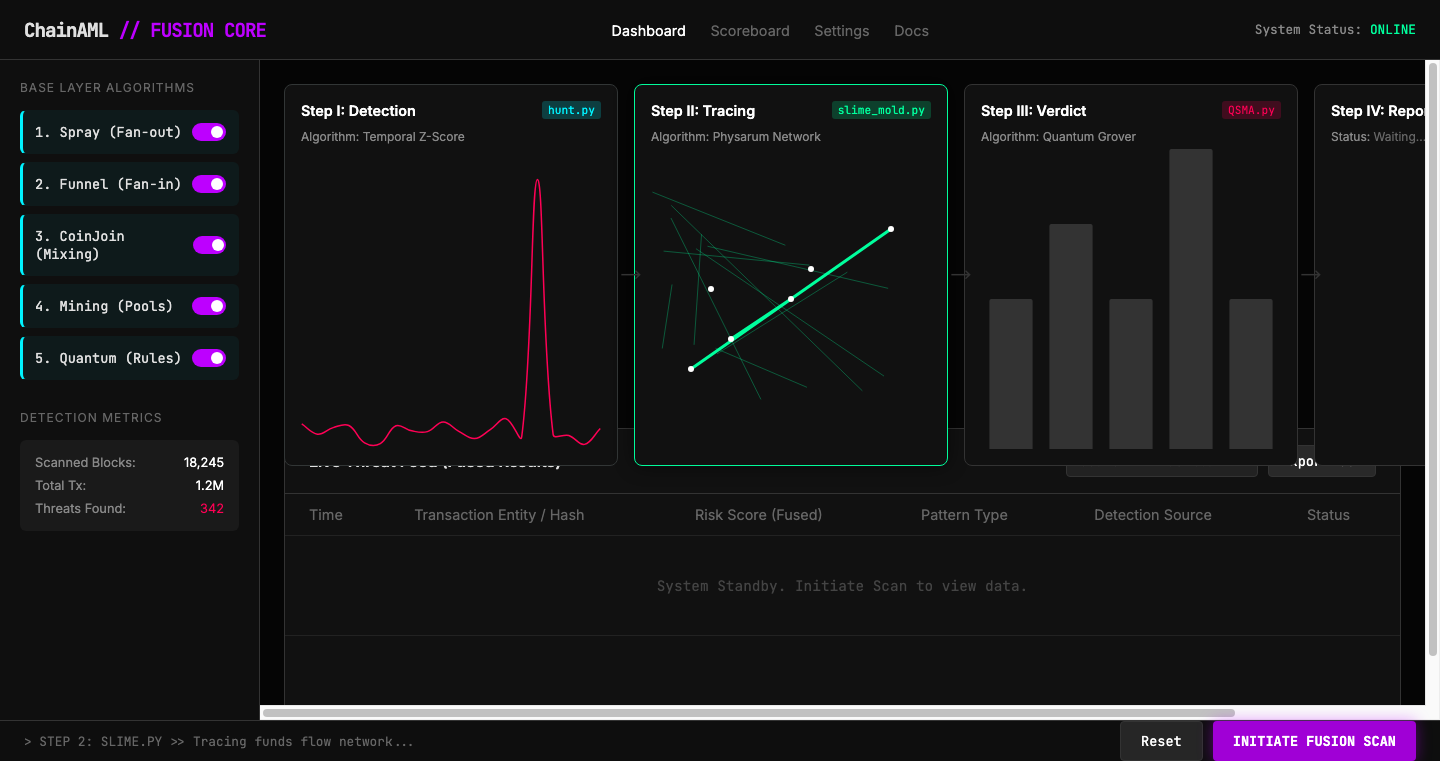
\includegraphics[width=0.9\linewidth]{step1.png}
  \caption{Step I：时间尖刺检测截图（占位）}
\end{figure}
\begin{figure}[h]
  \centering
  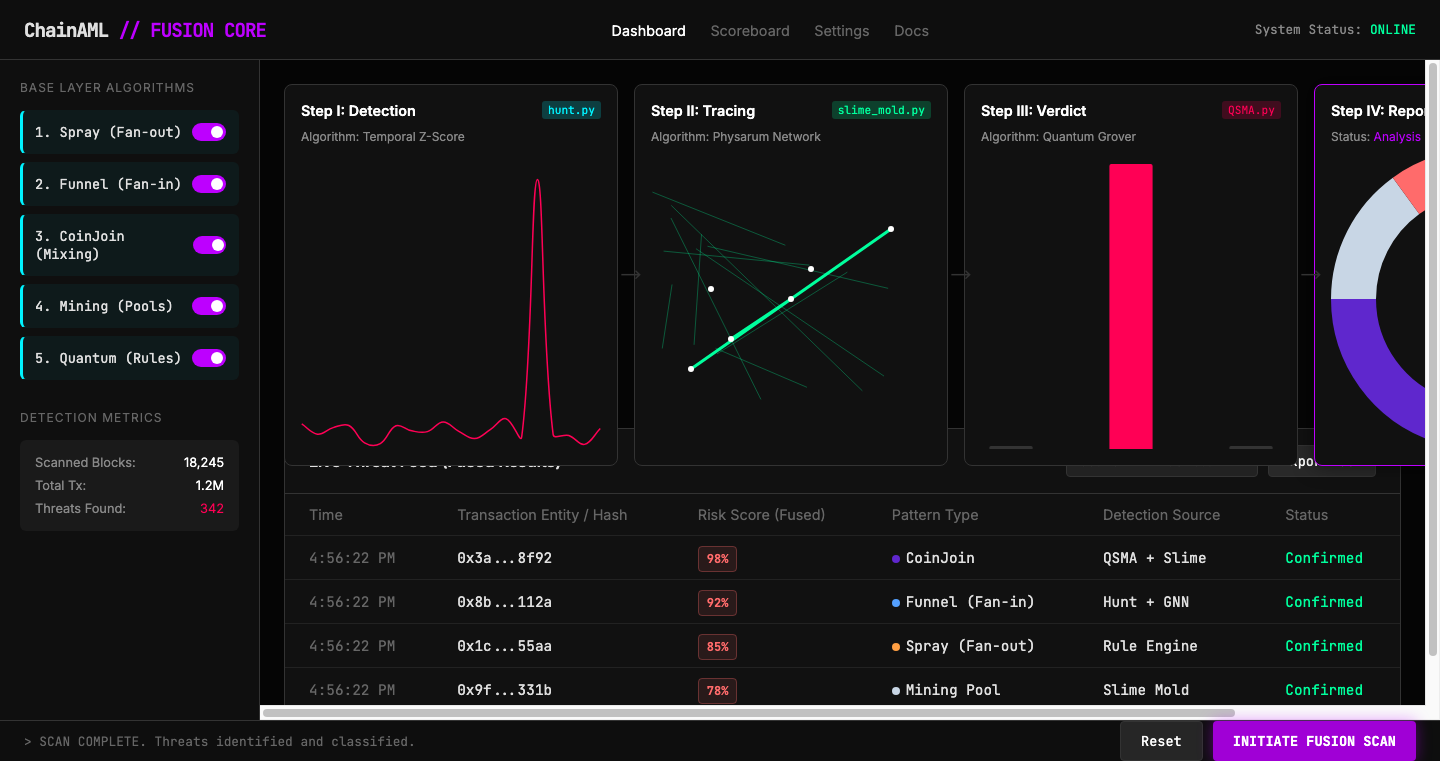
\includegraphics[width=0.9\linewidth]{step4_ring.png}
  \caption{Step IV：五类分类环图截图（占位）}
\end{figure}

\end{document}

